
\documentclass[10pt,a4paper]{article}
\usepackage{fontspec}
\setmainfont{Times New Roman}
\usepackage{graphicx}
\usepackage{array}
\setlength{\textwidth}{16.6cm}
\setlength{\oddsidemargin}{-0.9cm}
\setlength{\evensidemargin}{-0.9cm}
\setlength{\topmargin}{-1.75cm}
\setlength{\headheight}{0pt}
\setlength{\headsep}{0pt}
\setlength{\textheight}{25.2cm}
\setlength{\footskip}{0.9cm}
\setlength{\parindent}{0pt}
\setlength{\parskip}{3.6pt}
\linespread{1.06}
\widowpenalty=10000
\clubpenalty=10000
\makeatletter
\renewcommand\section{\@startsection{section}{1}{\z@}%
  {10pt plus 1pt minus 1pt}{3.5pt}{\normalfont\large\bfseries}}
\renewcommand\subsection{\@startsection{subsection}{2}{\z@}%
  {7pt plus 1pt minus 1pt}{2.5pt}{\normalfont\normalsize\bfseries}}
\makeatother
\begin{document}
\fontsize{10.5pt}{13pt}\selectfont

\begin{center}
{\LARGE\bfseries Selecting Reliable LLM Reasoning with Out-of-Fold Stacking of Answer-Shape and Arithmetic Evidence\par}
\vspace{6pt}
{\large Liangjinwei  $\cdot$  3036708414\par}
\vspace{2pt}
{\small\itshape DASE7506 Advanced Machine Learning Methods $\cdot$ Fall 2026  $\cdot$  Individual coursework (MP2)\par}
\end{center}
\vspace{3pt}
\begin{quote}
\small
\textbf{Abstract}\quad Each question in this task comes with four candidate solutions written by a language model, and only the final numeric answer of the chosen solution is graded. We build a CPU-only selector that never calls a language model at inference time. Six permutation-invariant base scorers --- text statistics, question-centred frozen embeddings, answer-shape features and arithmetic re-execution features --- are combined through a ten-fold out-of-fold score matrix and a Bradley--Terry meta-learner. On the official test bank the frozen system reaches 83.30\% (389/467), 14.14 points above plurality voting (69.16\%) and identical to the previous best stacker (83.30\%, also 389/467). On a pre-registered 355-question validation subset that mimics the test structure, it improves from 86.48\% to 88.17\%. The improvement comes from answer-shape evidence (+1.13 to +1.69 points) and does not transfer: the two systems disagree on 42 of 467 test questions yet get exactly the same number right. Analysis locates the residual difficulty in questions with a single correct candidate (69.30\% accuracy, versus 100\% when three candidates are correct), where wrong answers are arithmetically self-consistent and only a semantic reading of the question separates them from the right one. We report more than 45 falsified directions over eleven rounds and argue that, under the frozen-embedding and no-LLM constraints, the remaining errors are semantic rather than statistical.
\end{quote}
\vspace{-6pt}
{\small\itshape \textbf{Keywords:} candidate selection, verifier, out-of-fold stacking, Bradley--Terry, answer shape, GSM8K\par}
\vspace{4pt}
\section*{1 Introduction}
A language model asked a grade-school arithmetic question can return four solutions that all look plausible, use several correct-looking steps, and end with different numbers. The task studied here is to pick one of them. Each question supplies four candidate texts and a frozen 1024-dimensional representation of each candidate; the only thing graded is the final numeric answer of the chosen candidate, parsed by a fixed parser that accepts equivalent fractions and decimals. The language model is never available at evaluation time. We must decide, from the text and the frozen representations alone, which of four answers to trust.

The setting is deliberately adversarial. Every question has at least one correct candidate, several candidates may be correct, and the test bank is harder than the development splits: the mean number of correct candidates is 2.04 on test versus 3.03 on validation, and no test question has all four candidates correct (Section 3). A selector therefore cannot win by learning that ``the majority is usually right'': on the test bank plurality voting reaches only 69.16\%. Conversely, a solution may show a bad intermediate step yet land on the right final answer, so process-level correctness is not what the metric rewards.

We build a selector around a simple claim: the useful signal in a candidate is not its length or its confident wording, but the shape of its final answer relative to the numbers in the question, combined with a question-centred representation of the whole solution. Six base scorers are trained on disjoint folds of the training set and combined by an out-of-fold (OOF) score-level stacker that ranks the four candidates with a Bradley--Terry pairwise loss. The frozen system runs in pure NumPy on CPU, stores 60 KB of assets and scores the complete test bank in under four seconds on a laptop.

Our contributions are:

\begin{itemize}
\setlength{\itemsep}{1.5pt}
\setlength{\parskip}{0pt}
\item a frozen, CPU-only selector that reaches 83.30\% (389/467) on the official test bank and 88.17\% on a pre-registered 355-question validation subset, 14.14 points above plurality voting;
\item evidence that answer-shape features are the only new family that survives stacking (+1.13 points alone; the ensemble loses 1.41 points when they are removed), while arithmetic re-execution is absorbed by the evidence already present;
\item a clean measurement of OOF leakage: in-fold scores inflate training accuracy by 10.83 points and reduce validation accuracy by 2.54;
\item a negative result that we treat as central rather than incidental: the validation gain does not transfer. The deployed system and the previous best stacker disagree on 42 of 467 test questions and get exactly the same number right;
\item a map of more than 45 falsified directions over eleven rounds, with an accounting of their cost, which locates the ceiling in k = 1 questions where wrong answers are arithmetically consistent.
\end{itemize}
\vspace{2pt}
The rest of the report describes the data and metric (Section 3), the method (Section 4), the protocol (Section 5), results (Section 6), analysis and failures (Section 7), cost and reproducibility (Section 8), limitations (Section 9) and conclusions (Section 10).

\section*{2 Related Work}
Chain-of-thought prompting (Wei et al., 2022) made multi-step reasoning a standard output format for language models, and self-consistency (Wang et al., 2022) turned multiple sampled chains into a vote. Our plurality baseline is exactly that vote, applied to four fixed candidates. Trained verifiers (Cobbe et al., 2021) and process supervision (Lightman et al., 2023) instead learn a scorer over solutions or over individual steps; both require either a generator that can produce many candidates or step-level labels, and neither is available here. Test-time compute scaling (Snell et al., 2024) shows that the value of verifier-guided search depends on problem difficulty, which is consistent with our finding that the residual errors are concentrated in the hardest stratum.

The candidates and their frozen representations were produced with Qwen3-0.6B (Yang et al., 2025), but no model weights are distributed and we never run the model. The question is therefore not how to generate better candidates, but how much selection accuracy is attainable from frozen evidence under a 16 MiB asset budget and a 30 s CPU budget. Our negative results are a partial answer to that question: the signal exists, but its ceiling is set by what the frozen representation preserves, not by the capacity of the combiner.

\section*{3 Task, Data and Metric}
The data are 4,755 training, 798 validation and 467 test GSM8K questions (Cobbe et al., 2021); the candidate solutions and the 1024-dimensional whole-trace embeddings were generated offline with Qwen3-0.6B and are fixed. Each question has four candidates in a fixed order. References are supplied separately: training references for fitting, validation references for development and test references for final scoring only. The metric is selection accuracy: the chosen candidate’s final numeric answer is parsed and compared with the reference, and any correct candidate earns the point. Table 1 summarises the splits and the baselines that motivate the design.

\par\noindent\begin{minipage}{\textwidth}
\centering
{\footnotesize
\renewcommand{\arraystretch}{1.12}
\setlength{\tabcolsep}{3pt}
\begin{tabular}{@{}>{\raggedright\arraybackslash}p{2.90cm}>{\centering\arraybackslash}p{2.05cm}>{\centering\arraybackslash}p{2.73cm}>{\centering\arraybackslash}p{2.73cm}>{\centering\arraybackslash}p{2.39cm}>{\centering\arraybackslash}p{2.39cm}@{}}
\hline
\textbf{Split} & \textbf{Questions} & \textbf{Mean correct k} & \textbf{All four correct} & \textbf{Plurality vote} & \textbf{Parse failures} \\ \hline
train & 4,755 & 3.02 & 47.0\% & 85.3\% & 4.6\% \\
validation & 798 & 3.03 & 47.5\% & 86.2\% & 4.9\% \\
test & 467 & 2.04 & 0.0\% & 69.2\% & 5.9\% \\
\hline
\end{tabular}}
\par\vspace{2.5pt}
{\footnotesize\raggedright\textbf{Table 1.} Data and task statistics. k is the number of candidates whose parsed final answer equals the reference. Plurality vote picks the most frequent parsed answer. Parse failures are candidates whose final answer cannot be parsed. Test is much harder than validation and contains no question on which all four candidates are correct.\par}
\vspace{2pt}
\end{minipage}\par
\vspace{7pt}
Two properties of the data shape the whole study. First, k is unknown at prediction time and is not predicted: it is used only for post-hoc analysis, because k = 1 and k $\geq$ 2 questions are structurally indistinguishable from the candidate set alone. Second, full validation is a misleading development target: 379 of its 798 questions have all four candidates correct, so any reasonable selector scores highly there. We therefore pre-register a hard subset of the 355 validation questions whose four candidates contain at least two distinct parsed answers; this subset needs no labels to construct, and it reproduces the harness hard-subset accuracy exactly (313/355). It contains 114 questions with k = 1, 112 with k = 2 and 129 with k = 3.

The test bank is constructed to contain at least two distinct parseable answers per question, which is why the same definition is the right development proxy. One question on the hard subset is worth 0.28 points; differences below three questions (0.85 points) are noise, and we interpret every comparison in this report with that resolution in mind.

\section*{4 Method}
Figure 1 shows the deployed pipeline. It has four stages: feature extraction, six base scorers, an out-of-fold meta-feature matrix, and a Bradley--Terry meta-learner that returns the arg-max candidate.

\par\noindent\begin{minipage}{\textwidth}
\centering
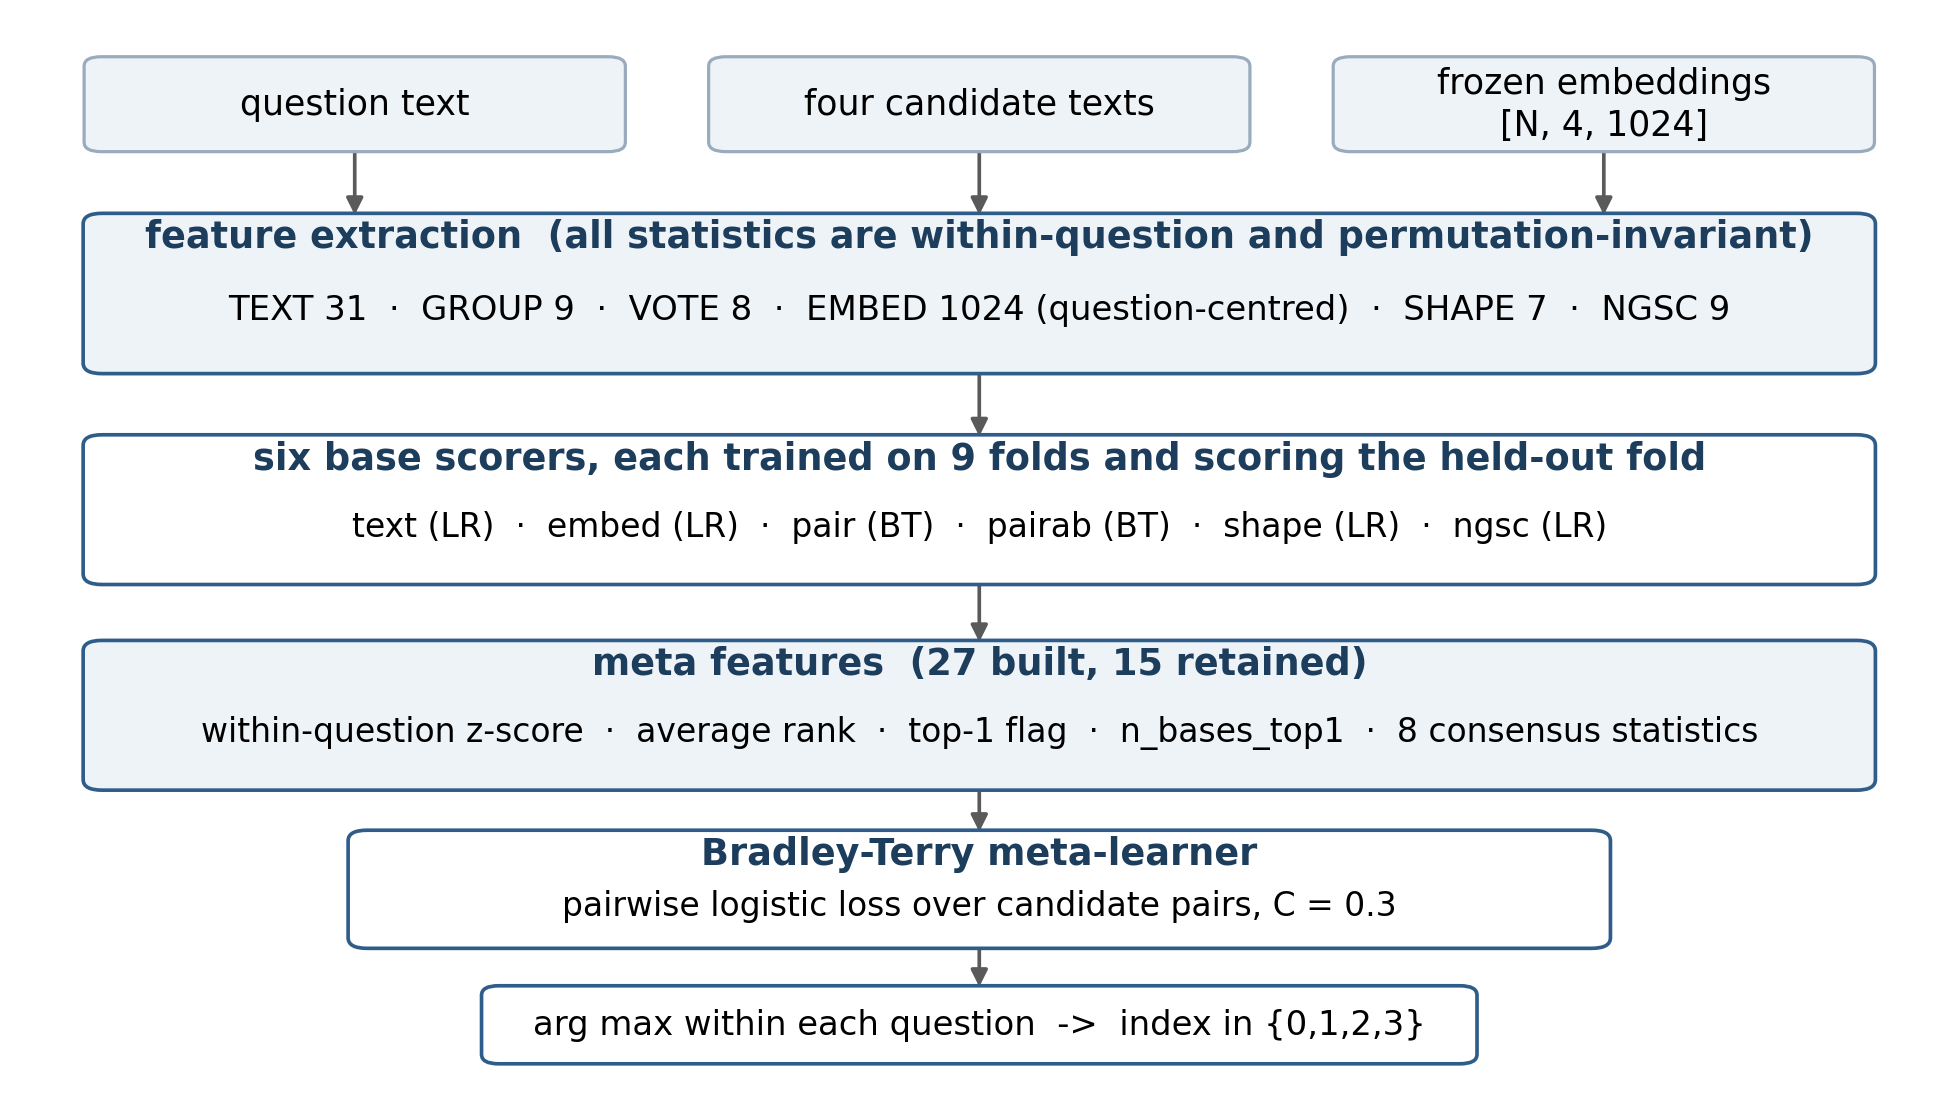
\includegraphics[width=15.6cm]{figures/fig1_pipeline.png}
\par\vspace{2pt}
{\footnotesize\raggedright\textbf{Figure 1.} The deployed selector. Every feature is a within-question statistic, so the candidate index is never used: under a random permutation of the four candidates, 0 of 798 validation answers change. The six base scorers are each trained out-of-fold; the meta-learner sees only their held-out scores.\par}
\vspace{2pt}
\end{minipage}\par
\vspace{7pt}
\subsection*{4.1  Permutation-invariant features}
All features are computed per question and per candidate without using the candidate index. The TEXT block (31 dimensions) describes a single solution: whether its answer parses, its sign, fraction, zero and integer indicators, log length, line and equation counts, number of numeric tokens, presence of \textbackslash{}boxed\{\} or \#\#\#\#, self-correction phrases, the position and count of the answer inside the text, digit density, and whether the last right-hand side of an equation equals the final answer. The GROUP block (9) adds within-question relatives: whether the answer is the mode, its share, the number of distinct parsed answers, length rank and deviation, and magnitude rank and deviation. The VOTE block (8) makes answer consensus explicit: vote share, count, mode membership, margin, ties, outlier and parse failure. The EMBED block is the frozen 1024-dimensional trace embedding, centred by subtracting the mean of the four candidates in the same question; this removes the question-level component that would otherwise act as a difficulty shortcut. The SHAPE block (7) describes the answer’s form: integer, fraction, negative, log magnitude, magnitude relative to the largest number in the question, density of the answer inside its own text, and how many question numbers equal it. The NGSC block (9) tests question-grounded self-consistency: whether the answer lies in the depth-0, depth-1 or depth-2 closure of the question’s numbers under +, $-$, $\times$ and $\div$, the smallest depth, the log closure size, and whether the LHS = RHS fragments in the text re-execute correctly and end at the final answer.

\subsection*{4.2  Six base scorers}
The six base scorers are deliberately diverse in both inputs and loss. Four are per-candidate logistic regressions with a binary correctness label; two operate on pairs of candidates with a Bradley--Terry loss. Table 2 lists them. Every scorer is trained on the 2,114 training questions that have 1 $\leq$ k $\leq$ 3 and at least two distinct parsed answers, with each question weighted by 1/k so that questions with many correct candidates do not dominate. Hyper-parameter C is chosen by question-level cross-validation on the training set.

\par\noindent\begin{minipage}{\textwidth}
\centering
{\footnotesize
\renewcommand{\arraystretch}{1.12}
\setlength{\tabcolsep}{3pt}
\begin{tabular}{@{}>{\raggedright\arraybackslash}p{2.01cm}>{\raggedright\arraybackslash}p{4.94cm}>{\raggedright\arraybackslash}p{6.59cm}>{\centering\arraybackslash}p{1.65cm}@{}}
\hline
\textbf{Base} & \textbf{Input blocks} & \textbf{Model and loss} & \textbf{C} \\ \hline
text & TEXT + GROUP & per-candidate logistic regression & 0.3 \\
embed & EMBED & per-candidate logistic regression & 0.01 \\
pair & TEXT + GROUP + EMBED & Bradley--Terry linear ranker & 0.03 \\
pairab & EMBED & Bradley--Terry linear ranker & 0.003 \\
shape & EMBED + SHAPE & per-candidate logistic regression & 0.003 \\
ngsc & NGSC & per-candidate logistic regression & 0.3 \\
\hline
\end{tabular}}
\par\vspace{2.5pt}
{\footnotesize\raggedright\textbf{Table 2.} The six base scorers of the deployed configuration (content4 + shape + ngsc). Each base model is fitted ten times, once per fold, so that the meta-learner never sees a score produced by a model that was trained on the same question.\par}
\vspace{2pt}
\end{minipage}\par
\vspace{7pt}
\subsection*{4.3  Out-of-fold stacking and the meta-learner}
We split the 2,114 training questions into ten folds. For each fold, every base scorer is fitted on the other nine folds and scores the held-out fold, producing an out-of-fold score matrix S of shape [N, 4, 6]. The meta-features (27 dimensions) are the within-question z-score, average rank and top-1 indicator of each base score, the number of bases that rank a candidate first, and eight consensus statistics. The deployed model keeps the 15 dimensions that the earlier meta-search selected: the six z-scores, the top-1 count, and the eight consensus statistics. A linear Bradley--Terry model is then fitted on candidate pairs:

\[ L_{BT} = -\sum_{q}\sum_{(i\succ j)} \log \sigma\left(s_{q,i}-s_{q,j}\right) + \lambda\|w\|^{2}, \]
where the sum runs over ordered pairs of candidates within each question. At prediction time the model scores the four candidates of a new question and returns the arg-max; the score of a candidate is its standardised meta-feature vector times w. The regularization strength C = 0.3 was chosen by question-level cross-validation on the OOF matrix, with a 0.2-point tie band and validation used only to break ties, as the protocol permits. Test references never enter training, feature construction, hyper-parameter search or model selection.

\subsection*{4.4  Design decisions and rejected alternatives}
Four decisions were forced by the evidence rather than chosen a priori. (i) SHAPE must be attached to EMBED, not to TEXT: the same feature block on text+group falls to 85.92\%, below the content-only baseline, while on embeddings it reaches 87.89\%. (ii) NGSC must be a separate base: attached to text it is absorbed and adds 0.00; as its own base it supplies the only dissenting signal in some failure cases, and its leave-one-out cost is +0.28. (iii) The two explicit vote bases are dropped: they collapse on k = 1 questions, and removing them raises k = 1 accuracy from 68.42\% to 69.30\% without changing k $\geq$ 2. (iv) The fusion is pairwise, not pointwise: a pointwise meta-learner on the same 15 features scores 84.51\% versus 88.17\% for the pairwise loss. Two further alternatives were rejected: a literal eight-base fusion (87.61\%) and shape attached to text (85.92\%).

\section*{5 Experimental Protocol}
Development uses the 355-question validation hard subset. The official test bank is evaluated once, after the configuration, hyper-parameters and files are frozen, using the supplied predict.py and score\_predictions.py. Test references are never used to train, tune, select, construct lookup tables or choose between schemes. Seventeen of the 33 schemes were eventually run on the test bank; each was scored once, and the report states explicitly when a test number is quoted from a scheme’s own record.

Training uses a single seed (20260916). All inference runs with four threads across OMP, OpenBLAS, MKL and NumExpr. The assets are the nine files in the checkpoint directory (six base models, the meta-learner, the configuration and the checksum list), whose SHA-256 hashes are recorded with the submission. Permutation invariance is checked by applying a fixed permutation [1, 2, 0, 3] to every validation question and re-running the frozen model: the chosen answers change for 0 of 798 questions, the chosen indices for 3 (exact ties among identical candidates), and the maximum score change is 1.8 $\times$ 10$^{-15}$.

Because the test references are public, repeated evaluation is a real risk. We mitigate it in three ways: selection was made on validation only; test was run only for schemes that improved the validation metric; and this report compares the deployed scheme with the previous best on the same frozen test predictions rather than re-tuning anything after seeing test.

\section*{6 Results}
Table 3 gives the main comparison. The deployed selector reaches 83.2976\% on the official test bank (389/467), 14.14 points above plurality voting (69.16\%, 323/467) and exactly equal to the previous best six-base stacker (83.30\%, 389/467). On validation it reaches 94.74\% overall and 88.17\% on the hard subset, against 86.48\% for the same-pipeline reproduction of the previous configuration, a gain of 1.69 points, or six questions.

\par\noindent\begin{minipage}{\textwidth}
\centering
{\footnotesize
\renewcommand{\arraystretch}{1.12}
\setlength{\tabcolsep}{3pt}
\begin{tabular}{@{}>{\raggedright\arraybackslash}p{3.84cm}>{\centering\arraybackslash}p{2.04cm}>{\centering\arraybackslash}p{2.45cm}>{\centering\arraybackslash}p{3.60cm}>{\centering\arraybackslash}p{1.63cm}>{\centering\arraybackslash}p{1.63cm}@{}}
\hline
\textbf{Method} & \textbf{Val full} & \textbf{Val hard (355)} & \textbf{Official test} & \textbf{Assets} & \textbf{Predict} \\ \hline
Plurality vote & 86.22\% & 69.01\% & 69.16\% (323/467) & 0 B & 0.02 s \\
Previous best stacker (s11) & 94.36\% & 87.32\% & 83.30\% (389/467) & 59.5 KB & 2.97 s \\
\textbf{Deployed (s16)} & \textbf{94.74\%} & \textbf{88.17\%} & \textbf{83.30\% (389/467)} & \textbf{60.1 KB} & \textbf{2.67 s} \\
\hline
\end{tabular}}
\par\vspace{2.5pt}
{\footnotesize\raggedright\textbf{Table 3.} Main results. The hard subset is the 355 validation questions with at least two distinct parsed answers. Test figures come from one frozen run of the official pipeline. The deployed method matches the previous best on test while improving the validation hard subset; the validation gain does not transfer.\par}
\vspace{2pt}
\end{minipage}\par
\vspace{7pt}
The equality on test is not an accident of rounding. The two systems choose different candidates on 42 of 467 questions, but the number they get right is identical (389 each), so they make different mistakes for the same score. This is the central negative result of the project and we return to it in Section 7.3.

Figure 2a explains where the validation gain comes from. On questions with three correct candidates both methods are at 100\%; on questions with two correct candidates the deployed method is slightly worse (93.75\% versus 94.64\%), but on the hardest stratum, k = 1, it improves from 21.05\% for plurality voting to 69.30\%, and from 64.03\% for the previous stacker. The k $\geq$ 2 total is unchanged at 234/241, so the gain is entirely a k = 1 gain. This matters because k = 1 is where the wrong answer is the majority and where arithmetic consistency cannot help.

\par\noindent\begin{minipage}{\textwidth}
\centering
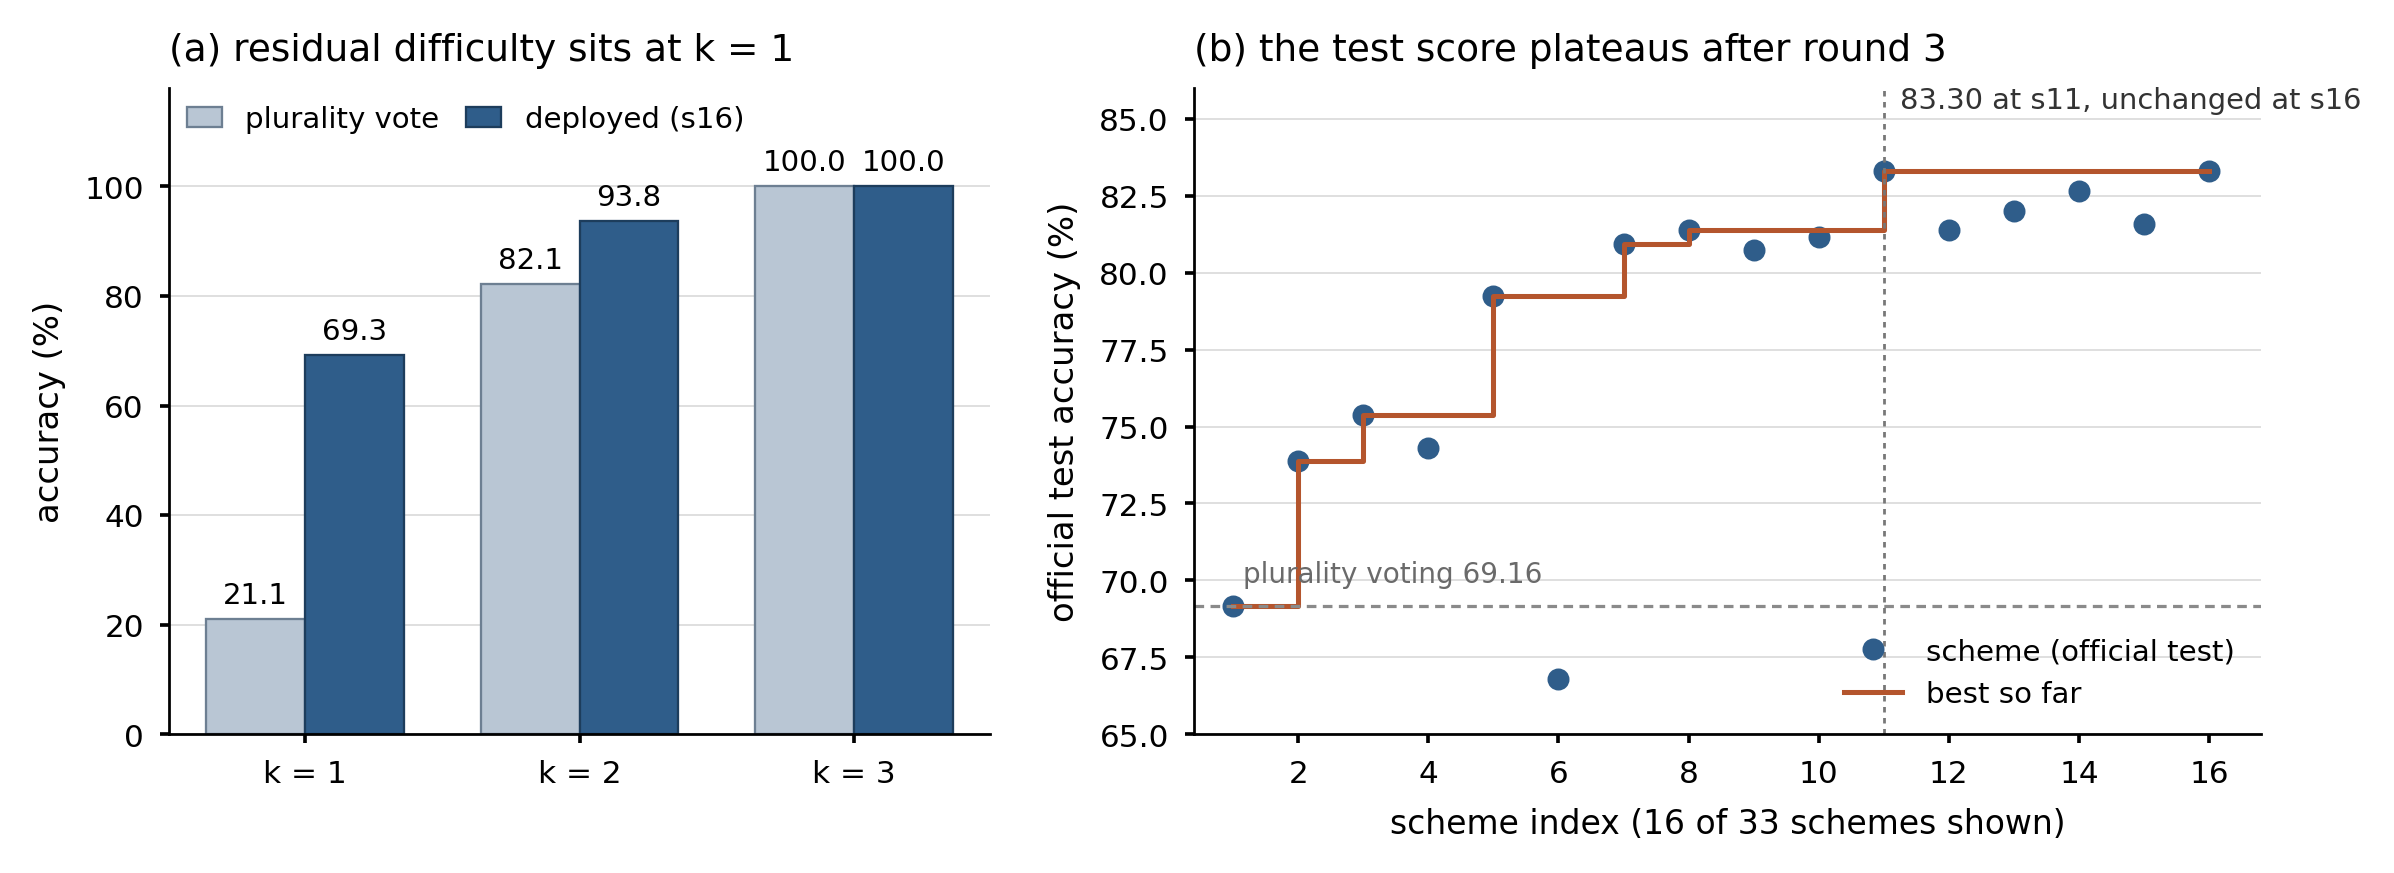
\includegraphics[width=16.0cm]{figures/fig2_evidence.png}
\par\vspace{2pt}
{\footnotesize\raggedright\textbf{Figure 2.} (a) Accuracy on the 355-question validation hard subset, split by k, the number of correct candidates. All of the improvement over the previous stacker is on k = 1; k $\geq$ 2 is unchanged in total. (b) Official test accuracy of the sixteen schemes of rounds 1--5 that were run on test. The best score rises from 69.16\% to 83.30\% in round 3 and then stays flat; schemes 17--32 were not run on test because they did not beat the validation gate.\par}
\vspace{2pt}
\end{minipage}\par
\vspace{7pt}
\section*{7 Analysis}
\subsection*{7.1  Ablations}
Table 4 isolates the contribution of every component. Panel A varies the base set. Adding SHAPE to the content-only four bases raises the hard subset from 86.76\% to 87.89\% (+1.13); adding NGSC alone leaves it unchanged (+0.00); adding both reaches 88.17\%. The literal eight-base fusion is worse (87.61\%) because the two vote bases hurt k = 2. Panel B removes one base at a time from the deployed set and retrains the meta-learner. Every base has a positive marginal, but SHAPE is the largest single contributor (+1.41), ahead of text and pair (+1.13 each), while NGSC contributes only +0.28. The difference between NGSC’s +0.00 when added alone and +0.28 when removed is not a contradiction: it is complementary only in the presence of SHAPE, and even then it is small.

\par\noindent\begin{minipage}{\textwidth}
\centering
{\footnotesize
\renewcommand{\arraystretch}{1.12}
\setlength{\tabcolsep}{3pt}
\begin{tabular}{@{}>{\raggedright\arraybackslash}p{6.38cm}>{\centering\arraybackslash}p{1.43cm}>{\centering\arraybackslash}p{1.26cm}>{\centering\arraybackslash}p{1.85cm}>{\centering\arraybackslash}p{1.43cm}>{\centering\arraybackslash}p{1.43cm}>{\centering\arraybackslash}p{1.43cm}@{}}
\hline
\textbf{Configuration} & \textbf{Bases} & \textbf{C} & \textbf{Val hard} & \textbf{k=1} & \textbf{k=2} & \textbf{k=3} \\ \hline
A. content only & 4 & 0.1 & 86.76\% & 64.03\% & 95.54\% & 99.22\% \\
A. content + SHAPE & 5 & 0.1 & 87.89\% & 68.42\% & 94.64\% & 99.22\% \\
A. content + NGSC & 5 & 0.1 & 86.76\% & 64.91\% & 94.64\% & 99.22\% \\
A. previous best configuration & 6 & 0.01 & 86.48\% & 64.03\% & 94.64\% & 99.22\% \\
\textbf{A. content + SHAPE + NGSC (deployed)} & \textbf{6} & \textbf{0.3} & \textbf{88.17\%} & \textbf{69.30\%} & \textbf{93.75\%} & \textbf{100\%} \\
A. literal eight-base fusion & 8 & 0.3 & 87.61\% & 68.42\% & 92.86\% & 100\% \\
B. drop text & --- & --- & 87.04\% & --- & --- & --- \\
B. drop embed & --- & --- & 87.32\% & --- & --- & --- \\
B. drop pair & --- & --- & 87.04\% & --- & --- & --- \\
B. drop pairab & --- & --- & 87.89\% & --- & --- & --- \\
B. drop SHAPE & --- & --- & 86.76\% & --- & --- & --- \\
B. drop NGSC & --- & --- & 87.89\% & --- & --- & --- \\
\hline
\end{tabular}}
\par\vspace{2.5pt}
{\footnotesize\raggedright\textbf{Table 4.} Ablations on the validation hard subset. Panel A varies the base set; Panel B removes one base from the deployed set and retrains the meta-learner. The deployed configuration is in bold. The previous-best row is a same-pipeline reproduction of scheme 11’s configuration (86.48\%); scheme 11 itself reported 87.32\%. Panel B has no per-k breakdown because only the aggregate was recorded for those runs.\par}
\vspace{2pt}
\end{minipage}\par
\vspace{7pt}
Two further controls are worth stating because they are easy to get wrong. First, the encoding of new evidence matters more than the evidence itself: the same SHAPE block on text+group scores 85.92\%, below the content baseline, while on embeddings it scores 87.89\%. Second, out-of-fold construction is not cosmetic. Fitting the meta-learner on in-fold base scores inflates its training accuracy from 83.16\% to 93.99\% (+10.83) and lowers validation accuracy from 88.17\% to 85.63\% ($-$2.54). The leak makes the meta-learner believe the bases are nearly perfect and mis-weights them; OOF both removes the illusion and improves generalisation.

\subsection*{7.2  Failure cases and uncertainty}
The deployed system makes 42 errors on the 355-question hard subset. Three of them are unanimous: all six bases pick the same wrong candidate. In the square-dancing question the parsed answers are [48, 48, 45, 2] and the gold answer is 2; every base picks 48, because the wrong solution computes 94 $-$ 46 consistently but starts from the wrong base. In the pie question the parsed answers are [5, 5, 240, 4] and every base picks 5. A non-unanimous failure appears in the paperclip question, where the parsed answers are [9, 17, 17, 17] and the gold answer is 9: the three wrong candidates all compute 8 + 2 + 7 = 17, SHAPE sides with the majority because 17 is also an integer, also reachable and also arithmetically consistent, and NGSC is the only base that dissents, but it is outvoted. In each case the wrong answer is arithmetically self-consistent; what fails is the reading of the question. These are not statistical errors that more capacity would fix; they are semantic misreadings with correct arithmetic.

Uncertainty is not a usable escape hatch. A calibration probe on the pairwise model recorded an expected calibration error of 0.270 and a Spearman correlation of 0.06 between confidence rank and correctness; the highest-margin quintile was not the most accurate. Ablation-based abstention would therefore discard good and bad questions at similar rates. This is consistent with the k = 1 analysis: the model is confident precisely where the majority is confidently wrong.

\subsection*{7.3  Why the test score did not move}
The validation gain is real but small, and it sits on the wrong side of the test boundary. Three observations explain the plateau. First, an oracle that could pick the best base scorer per question would score 94.09\% on the hard subset with the original six bases and 95.78\% with all eight; the deployed 88.17\% is 5.9 points below the six-base oracle, so the residual gap is one of selection rather than a missing base family. Second, the remaining headroom is concentrated in k = 1: across the twelve schemes analysed in round 3, the oracle over schemes reaches 84.21\% on k = 1 while the best single scheme reaches 69.30\%, and 20 of the 355 questions are solved by no scheme at all. Third, k = 1 and k = 3 are structurally identical from the candidate set: both present a 3-vs-1 split of parsed answers, and only a reading of the question distinguishes a wrong majority from a right one. A frozen whole-trace embedding preserves topic and style; it does not preserve the computation.

The 42-question disagreement with the previous stacker is consistent with this account. The two systems use different evidence and therefore make different k = 1 errors, but neither has access to the semantic relation that would resolve them, so the errors exchange one for one. This is why we report the test result as a draw rather than as an improvement: at this resolution, 42 different choices and 389 correct answers are the signature of a ceiling, not of noise.

\subsection*{7.4  What we tried, and what it cost}
Table 5 summarises eleven rounds and 33 schemes. Rounds 1--3 produced the only real progress: pairwise scoring, question-centred embeddings and OOF stacking moved the test score from 69.16\% to 83.30\%. Rounds 4--5 added numeric reachability, answer shape and arithmetic re-execution; they improved validation but not test. Rounds 6--10 tested conditional stacking, MLP capacity, end-to-end rankers, replication-aware voting, mid-consensus evidence, lexical duplicates, a from-scratch text encoder and weak-evidence bundles; none beat the validation gate, so none was run on test. Round 11 added a conservative hand-written arithmetic solver that overrides the stacker only when the question states an explicit recurrence or chase relation; it corrected one validation question (314/355) and changed no test prediction (389/467).

\par\noindent\begin{minipage}{\textwidth}
\centering
{\footnotesize
\renewcommand{\arraystretch}{1.12}
\setlength{\tabcolsep}{3pt}
\begin{tabular}{@{}>{\centering\arraybackslash}p{1.50cm}>{\centering\arraybackslash}p{2.06cm}>{\raggedright\arraybackslash}p{9.57cm}>{\centering\arraybackslash}p{2.06cm}@{}}
\hline
\textbf{Round} & \textbf{Schemes} & \textbf{Main directions} & \textbf{Best test} \\ \hline
1 & 01--08 & voting, text/GBDT probes, embedding probe, relative features, pairwise, hybrid & 81.37\% \\
2 & 09--10 & distribution-aligned pairwise, k = 1 detector & 81.16\% \\
3 & 11--13 & OOF stacking, k = 1 specialist, set verifier & 83.30\% \\
4 & 14--15 & numeric reachability, new-evidence search & 82.66\% \\
5 & 16 & stacker + answer shape + arithmetic re-execution & 83.30\% \\
6--10 & 17--32 & conditional stacking, MLP capacity, end-to-end ranker, replication-aware voting, mid-consensus, lexical duplicates, scratch encoder, weak-evidence bundle & not run \\
11 & 33 & conservative semantic arithmetic guard & 83.30\% \\
\hline
\end{tabular}}
\par\vspace{2.5pt}
{\footnotesize\raggedright\textbf{Table 5.} Search log. Each round was evaluated on the validation hard subset; test was run only when a scheme improved the validation metric. Rounds 6--10 produced no validation gain and were therefore not run on test. The table is the cost side of the cost--benefit argument: twenty schemes after round 3 did not improve the test score.\par}
\vspace{2pt}
\end{minipage}\par
\vspace{7pt}
The deployed method is cheap; the search that produced it was not. A full training run takes about six minutes on CPU (63.8 s when the base-score cache is warm), each scheme requires feature extraction over 4,755 questions and a ten-fold refit, and the eleven rounds together cost far more than the four seconds of inference they eventually deliver. The last twenty schemes are not justified by the measured test gain. What is justified is the fusion step: OOF stacking was the single largest improvement in the project (+1.93 test from round 2 to round 3) and costs nothing at inference beyond a linear model.

\section*{8 Cost, Constraints and Reproducibility}
The submitted checkpoint contains nine files and 60,125 bytes in total, 0.36\% of the 16 MiB budget: six base-model files, meta.npz, config.json and SHA256SUMS.txt. Every file’s SHA-256 hash is recorded in the checkpoint directory. Inference imports only NumPy (scikit-learn is used for training only), runs on CPU, and is deterministic. On the local machine (Intel Core i5-11300H, 4 cores / 8 threads, 4 threads pinned via OMP, OpenBLAS, MKL and NumExpr) a fresh prediction process on the 467-question test bank takes 3.4 s wall-clock and the independent scoring process 0.4 s, 3.8 s in total including interpreter startup. The reference Xeon Platinum 8457C was not available; the recorded in-process prediction time is 2.67 s and the official scorer reports 0.048 s, both far below the 30 s limit. A peer reproducing on the reference machine should expect a similar margin, but the eligibility figure remains the reference machine’s.

Training is a ten-fold OOF fit on 2,114 questions with seed 20260916; it takes 63.8 s with cached base scores and about six minutes cold on CPU. The environment recorded during method development was Python 3.13.12 with NumPy 2.5.4 and scikit-learn 1.9.1. That interpreter was no longer available when this report was written, so the final verification was run with Python 3.11.4 and NumPy 1.26.4; the frozen model reproduced the archived test predictions exactly, with 0 of 467 chosen indices different and the official scorer returning 389/467. The reproduction therefore does not depend on the minor version of the linear-algebra library.

Reproduction commands (from code/, with the four thread variables set to 4):

\par\noindent\begin{minipage}{\textwidth}
\begin{verbatim}
python check_data.py
python predict.py --method ../solutions/16_final_fusion/method.py \
    --checkpoint ../solutions/16_final_fusion/artifacts \
    --split test --output runs/test-predictions.json
python score_predictions.py --split test \
    --predictions runs/test-predictions.json --output runs/test-score.json
\end{verbatim}
\end{minipage}\par
\vspace{2pt}
The official test JSON, the validation JSON, the ablation record, the failure list and the checkpoint hashes are submitted with the code. The code version and the checkpoint are identified by the same commit. Data and attribution are unchanged: GSM8K provides the questions and references (Cobbe et al., 2021), Qwen3-0.6B produced the candidates and embeddings (Yang et al., 2025), and no model weights are redistributed.

AI disclosure. AI coding assistants were used to draft implementation code, analysis scripts and parts of this manuscript. The headline validation and test numbers were re-run against the official evaluator before submission, and the final test prediction was produced by a fresh process and compared with the archived prediction (0/467 index changes); the ablation and diagnostic numbers are taken from the recorded experiment files shipped with the code. No reported result is copied from an external source.

\section*{9 Limitations and Threats to Validity}
The main limitation is resolution. The validation hard subset has 355 questions, so one question is 0.28 points and the +0.85 validation gain over the previous report is three questions; it is not statistically strong. The test bank is harder than validation (mean k 2.04 versus 3.03, no question with four correct candidates), so a validation gain can fail to transfer even when it is real, as happened here. A second limitation is coverage: only one seed was run, no external audit bank was available, and the frozen whole-trace embedding was produced by a 0.6B model. The representation preserves topic and style but not the computation, which is exactly the information needed for k = 1 questions. Third, the test references were observed for seventeen schemes. Selection was made on validation and each scheme was scored once, but repeated observation is still a threat to the purity of the test estimate. Finally, the resource measurements were taken on a different CPU from the reference machine, and the training cost of the search (33 schemes) is much larger than the inference cost of the submission.

\section*{10 Conclusion}
The frozen selector reaches 83.30\% on the official test bank, 14.14 points above plurality voting and equal to the strongest previous stacker. The honest summary is a draw on test and a small, well-localised win on validation: answer shape is the only new evidence family that survives stacking, arithmetic re-execution is absorbed, and the residual errors are semantic misreadings with correct arithmetic. Table 6 states our answers to the five research questions posed in the assignment guide.

\par\noindent\begin{minipage}{\textwidth}
\centering
{\footnotesize
\renewcommand{\arraystretch}{1.12}
\setlength{\tabcolsep}{3pt}
\begin{tabular}{@{}>{\raggedright\arraybackslash}p{3.99cm}>{\raggedright\arraybackslash}p{8.93cm}>{\centering\arraybackslash}p{2.28cm}@{}}
\hline
\textbf{Research question} & \textbf{Answer} & \textbf{Evidence} \\ \hline
Does reading the reasoning help? & Yes, but through the answer rather than the steps: text statistics alone reach 78.03\%, centred embeddings 82.82\%, shape plus embedding 84.51\%, and stacking 88.17\%. Re-executing the equations adds nothing once the stacker exists. & Table 4 \\
What makes a wrong answer convincing? & Arithmetic consistency and agreement. In 3 of 42 failures every base agrees; the wrong answer is usually reachable and internally consistent. Length is the only weak surface cue and it is not enough. & Section 7.2 \\
Should a solution be judged on its own? & No. The gain comes from within-question relative meta-features and a pairwise loss; a pointwise meta-learner on the same features scores 84.51\% versus 88.17\%. & Table 4 \\
Can the method recognise its own uncertainty? & Not usefully. Calibration is poor (ECE 0.270) and confidence rank is nearly uncorrelated with correctness ($\rho$ = 0.06); abstention would not help. & Section 7.2 \\
When does more computation pay off? & Once, at fusion: OOF stacking is the largest single gain (+1.93 test). After that, about twenty more schemes and more than 45 directions produced 0.00 test gain; extra arithmetic is cheap but worthless. & Table 5 \\
\hline
\end{tabular}}
\par\vspace{2.5pt}
{\footnotesize\raggedright\textbf{Table 6.} Answers to the five research questions in the assignment guide.\par}
\vspace{2pt}
\end{minipage}\par
\vspace{7pt}
What would break the ceiling? Not more features of the same kind. The evidence points to three requirements: step-level labels so that a verifier can learn from intermediate reasoning rather than from the final answer; a larger validation bank, because 355 questions cannot resolve one-to-three-question differences; and a stronger or accessible generator, because the frozen 0.6B representation does not encode the computation. Within the rules of this assignment, the ceiling is best described as semantic: the method can tell a plausible answer from an implausible one, but not a well-argued wrong reading from a right one. That negative result is, we think, the most useful thing this project has to report.

\section*{References}
\begin{list}{}{%
\setlength{\leftmargin}{0.65cm}
\setlength{\itemindent}{-0.65cm}
\setlength{\itemsep}{2pt}
\setlength{\parsep}{0pt}
\footnotesize}
\item Cobbe, K., Kosaraju, V., Bavarian, M., Chen, M., Jun, H., Kaiser, L., Plappert, M., Tworek, J., Hilton, J., Nakano, R., Hesse, C., \& Schulman, J. (2021). Training verifiers to solve math word problems. arXiv preprint arXiv:2110.14168. https://arxiv.org/pdf/2110.14168
\item Lightman, H., Kosaraju, V., Burda, Y., Edwards, H., Baker, B., Lee, T., Leike, J., Schulman, J., Sutskever, I., \& Cobbe, K. (2023). Let’s verify step by step. arXiv preprint arXiv:2305.20050. https://arxiv.org/pdf/2305.20050
\item Snell, C., Lee, J., Xu, K., \& Kumar, A. (2024). Scaling LLM test-time compute optimally can be more effective than scaling model parameters. arXiv preprint arXiv:2408.03314. https://arxiv.org/pdf/2408.03314
\item Wang, X., Wei, J., Schuurmans, D., Le, Q., Chi, E., Narang, S., Chowdhery, A., \& Zhou, D. (2022). Self-consistency improves chain of thought reasoning in language models. arXiv preprint arXiv:2203.11171. https://arxiv.org/pdf/2203.11171
\item Wei, J., Wang, X., Schuurmans, D., Bosma, M., Ichter, B., Xia, F., Chi, E., Le, Q., \& Zhou, D. (2022). Chain-of-thought prompting elicits reasoning in large language models. arXiv preprint arXiv:2201.11903. https://arxiv.org/pdf/2201.11903
\item Yang, A., Li, A., Yang, B., Zhang, B., Hui, B., Zheng, B., Yu, B., Gao, C., Huang, C., Lv, C., Zheng, C., Liu, D., Zhou, F., Huang, F., Hu, F., Ge, H., Wei, H., Lin, H., Tang, J., $\ldots$ Qiu, Z. (2025). Qwen3 technical report. arXiv preprint arXiv:2505.09388. https://arxiv.org/pdf/2505.09388
\end{list}
\end{document}